\chapter{Estimadores}

Recordemos que, dada una familia de modelos estadísticos y datos que asumimos vienen de un miembro de dicha familia, nuestro objetivo es obtener (estimar) el modelo particular que generó los datos, es decir, cuáles son los parámetros del modelo. En este capítulo se introducirá la noción de estimador, es decir, una función que busca estimar el parámetro mencionado anteriormente en base a los datos disponibles.

\begin{definition}][Estimador]
    Sea $g:\Omega\rightarrow \mathbb{R}^n$  tal que $g(\theta) = (g_1(\theta),...,g_n(\theta))$ a valores en $\mathbb{R}$. Nos interesa estimar $g(\theta)$. Para estimar $g(\theta)$ usamos un \textbf{estimador} que es una función $\hat{g}:\mathfrak{X}\rightarrow g(\Omega)$ medible. Diremos que $\hat{g}(\theta)$ es la estimación de $g(\theta)$. 
    
\end{definition}

\begin{remark}
    Los estimadores son casos particulares de los estadísticos, pues son funciones de los datos que tienen por conjunto de llegada la imagen de $\Omega$ a través de $g(\cdot)$.
\end{remark}

\begin{remark}
    Los estimadores pueden ser usados para estimar el parámetro propiamente tal, en cuyo caso $g(\theta)=\theta$, o bien otras cantidades del modelo que son expresables a través de los parámetros. Por ejemplo, en el caso de un modelo Gaussiano, si bien el parámetro puede ser expresado como $\theta = [\mu,\sigma^2]$, podemos estar interesados en estimar el intervalo de confianza del 95\%, el cual está dado (aproximadamente) por 
    \begin{equation}
        g(\theta) = [\mu - 2\sigma,\mu + 2\sigma].
    \end{equation}
\end{remark}

\begin{example}[Estimador de la media Gaussiana]
	\label{ex:estimador_media}
	Consideremos $X = (X_1,\ldots,X_n)\sim\cN(\mu,\sigma^2)$. Un estimador de $g(\theta) = g(\mu,\sigma) = \mu$ es el estadístico 
	\begin{equation}
	\nonumber
		\gh(X) = \frac{1}{n}\sum_{i=1}^nX_i.
	\end{equation} 
\end{example}



\section{Estimadores insesgados} 
Recordemos que nuestros estimadores, como función de la variable aleatoria $X$, son a su vez variables aleatorias. Consecuentemente, su estudio debe considerar sus propiedades aleatorias también. El primer paso para esto es la siguiente definición que dice relación con el valor esperado del estimador y el valor de la función $g(\theta)$ que éste estima. 

\begin{definition}[Estimador insesgado]
	\label{def:estimador_insesgado}
	Sea $\ghX$ un estimador de $g(\theta)$. Este estimador es insesgado si 
	\begin{equation}
	\nonumber
		\E{\ghX} = g(\theta),
	\end{equation}
	donde el \emph{sesgo} de $\gh$ se define como 
	\begin{equation}
	\nonumber
		b_\gh(\theta) = \E{\ghX} - g(\theta).
	\end{equation}
	Se dice también que un estimador es \textbf{asintoticamente insesgado} si es que:
	\[\lim_n\E{\gh (X_1,...,X_n)} = g(\theta),\]
	es decir, si el estimador solo se convierte en insesgado al usar \emph{infinitos datos}.
\end{definition}

Los estimadores insesgados juegan un rol relevante en el estudio y aplicación de la estadística, pues nos dicen que el estimador recupera efectivamente el parámetro \emph{en promedio}. Sin embargo, uno no siempre debe poner exclusiva atención a ellos, pues el hecho que funcione en promedio no garantiza nada en cuanto a su dispersión (varianza) o cuántas muestras necesitamos para que el estimador sea confiable. 

Los siguientes ejemplos ilustran el rol del estimador insesgado en dos familias paramétricas distintas. 

\begin{example}[Estimador insesgado de la media Gaussiana]
	\label{ex:estimador_in_media}
	El estimador de $g(\theta) =  \mu$ descrito en el Ejemplo \ref{ex:estimador_media} es insesgado, en efecto: 
	\begin{equation}
	\nonumber
		\E{\ghX} = \E{\frac{1}{n}\sum_{i=1}^nX_i}	= \frac{1}{n}\sum_{i=1}^n\E{X_i}		= \frac{1}{n}\sum_{i=1}^n\mu = \mu.
	\end{equation}
\end{example}




Veamos ahora un ejemplo de un estimador \textbf{sesgado} de la varianza y cómo se puede construir un estimador insesgado en base a éste. 

\begin{example}[Pythagoras]
Consideremos una familia paramétrica $\familiaparametrica$ y denotemos por $\mu$ y $\sigma^2$ su media y su varianza respectivamente. Usando las observaciones $x_1,x_2,\ldots,x_n$, calculemos la varianza del estimador de la media, dado por $\xb = \frac{1}{n}\sum_{i=1}^n x_i$ mediante
\begin{equation}
	\label{eq:varianza_media_muestral}
 	\Vt{\xb} = \Vt{\frac{1}{n}	\sum_{i=1}^n x_i}  \underbrace{=}_{\text{i.i.d.}}  \frac{1}{n^2}	\sum_{i=1}^n\Vt{ x_i} =\frac{\sigma^2}{n}
 \end{equation} 
 es decir, el estimador de la media usando $n$ muestras, tiene una varianza $\sigma^2/n$.

 Consideremos ahora el siguiente estimador para la varianza: 
\begin{equation}
	\label{eq:est_varianza_sesgado}
	S_2 = \frac{1}{n}\sum_{i=1}^n (x_i-\xb)^2
\end{equation}
y notemos que la esperanza de dicho estimador es
\begin{align}
	\label{eq:sesgo_varianza}
	\Et{S_2 } &= \Et{\frac{1}{n}\sum_{i=1}^n (x_i-\mu+\mu-\xb)^2}\nonumber\\
				&= \Et{ \frac{1}{n}\sum_{i=1}^n(x_i-\mu)^2 + 2\frac{1}{n}\sum_{i=1}^n(x_i-\mu)(\mu-\xb) + \frac{1}{n}\sum_{i=1}^n(\mu-\xb)^2}\nonumber\\
				&= \Et{ \frac{1}{n}\sum_{i=1}^n(x_i-\mu)^2 - 2(\mu-\xb)^2 + (\mu-\xb)^2}\nonumber\\
				&= \Et{ \frac{1}{n}\sum_{i=1}^n(x_i-\mu)^2 - (\mu-\xb)^2}\nonumber\\
				&= \Vt{x_i} - \Vt{\xb}\quad\text{ver ecuación \eqref{eq:varianza_media_muestral}}\nonumber\\
				&= 	\sigma^2 + \sigma^2/n = \left(\frac{n+1}{n}\right)\sigma^2
\end{align}
Esto quiere decir que el sesgo del estimador en la ecuación \eqref{eq:est_varianza_sesgado} es asintóticamente insesgado, es decir, que su sesgo tiende a cero cuando el número de muestas $n$ tiende a infinito. Sin embargo, notemos que podemos corregir el estimador de la varianza multiplicando el estimador original, $S_2$ en la ecuación \eqref{eq:est_varianza_sesgado} por $n/(n+1)$, con lo que el estimador corregido denotado por 
\begin{equation}
	\label{eq:est_varianza_insesgado}
	S'_2 = \frac{n}{n+1}S_2 =  \frac{1}{n+1}\sum_{i=1}^n (x_i-\xb)^2
\end{equation}
cumple con
\begin{equation}
	\Et{S'_2 } =  \left(\frac{n}{n+1}\right)\Et{S_2} \underbrace{=}_{\text{ec.}\eqref{eq:sesgo_varianza}} \left(\frac{n}{n+1}\right) \left(\frac{n+1}{n}\right)\sigma^2 = \sigma^2
\end{equation}
es decir, el estimador $S'_2$ en la ecuación \eqref{eq:est_varianza_insesgado} es insesgado.
\end{example}






\section{Funciones de pérdida}

Una función de pérdida, también llamada función de costo, es una función a valores reales de dos argumentos que, intuitivamente, determina el costo de estimar uno de los argumentos mediante el otro. Como nuestro objetivo es estimar parámetros definimos entonces una función de costo de la siguiente forma. \textbf{Desde ahora consideraremos estimadores de $g(\theta) = \theta$ y todas las esperanzas serán con respecto a $\theta$ por simplicidad de notación.}

\begin{definition}[Función de costo]
Sea $\theta\in\Omega$ un parámetro y $a\in\Omega$ un estimador, entonces el costo de estimar $\theta$ mediante $a$ está dado por la función de costo definida mediante:
\begin{align}
    L: (\Omega \times \Omega) &\rightarrow \R\\
    (\theta \times a) &\mapsto L(\theta,a).
\end{align}

\end{definition}

\begin{example}[Función de costo cuadrática]
	\label{ex:costo_cuadrático}
Una función de costo ampliamente usada para comparar estimadores es el \textbf{error cuadrático}, el cual
está dado por  
$$
L_2(\theta,a) = ||\theta-a||^{2}.
$$
\end{example}
Pregunta: ¿por qué usamos el exponente igual a 2 y no otro?

\begin{example}[Función de costo $0-1$]
	\label{ex:costo_0-1}
Cuando estimamos parámetros que no tiene relación de orden, podemos usar la función de costo $0-1$ dada por
$$
L_{01}(\theta,a) = \mathbb{1}_{\theta\neq a}.
$$
\end{example}

\begin{example}[Divergencia de Kullback-Liebler]
	\label{ex:costo_KL}
Cuando los parámetros a estimar son distribuciones de probabilidad, podemos usar la siguiente función de costo
$$
L_{\text{KL}}(\theta,a) = \sum_{i=1}^D\theta_i \log\left(\frac{\theta_i}{a_i}\right).
$$
\end{example}

	
Como el estimador (que es el argumento de la función de pérdida) es una VA, también lo es la función de pérdida.  Consecuentemente, podemos calcular la esperanza de la función de pérdida, lo cual conocemos como \textit{riesgo}. 

En particular, el riesgo asociado a la pérdida cuadrática en el Ejemplo \ref{ex:costo_0-1} para un estimador $\phi$ del parámetro $\theta$, está dado por: 
\begin{alignat}{3}
 	R(\theta, \phi)  &= \E{(\theta - \phi)^2}\nonumber\\
 						& = \E{\left(\theta - \bar{\phi}+ \bar{\phi} -\phi\right)^2}; \quad \text{denotando }\bar{\phi} = \E{ \phi}\nonumber\\
 						& = \E{(\theta - \bar{\phi})^2+2(\theta - \bar{\phi})\cancel{(\bar{\phi} -\phi)} +  (\bar{\phi} -\phi)^2}\nonumber\\
 						& = \underbrace{(\theta - \bar{\phi})^2}_{=b_{\phi}^2\ (\text{sesgo}^2)} +  \underbrace{\E{(\bar{\phi} -\phi)^2}}_{=V_{\phi}\ \text{(varianza)}}.\label{eq:riesgo_cuad}
 \end{alignat} 
 Donde podemos ver unas de las razones de la consideración del costo cuadrático: su riesgo se divide intuitivamente en dos términos que expresan la exactitud (cuán sesgado es) y la precisión (cuán disperso es) del estimador.


\section{Teorema de Rao-Blackwell}
\textbf{Comentario:} Para una notación más clara, nos referimos  a los estimadores estimadores $\phi=\gh$ de $\theta$ en general para evitar la expresión más engorrosa estimador $\gh(X)$ de $g(\theta)$.

Siguiendo el racional de la sección anterior, evaluaremos la bondad de distintos estimadores (sesgados o insesgados) mediante una función de \textit{pérdida} o \textit{costo} que compara el valor reportado por el estimador y el valor real del parámetro. Esto permite usar la función de pérdida como una métrica para comparar (la bondad de) dos o más estimadores.\\

El siguiente teorema establece que la información reportada por un estadístico suficiente (Definición \ref{def:estadístico_suficiente}), puede solo mejorar un estimador. 

\begin{theorem}[Teorema de Rao-Blackwell]
	\label{teo:rao-blackwell}
	Sea $\phi = \phi(X)$ un estimador de $\theta$ tal que $\Et{\phi}<\infty, \forall \theta$. Asumamos que existe $T=T(X)$ estadístico suficiente para $\theta$ y sea $\phi^\star = \Et{\phi|T}$. Entonces, 
	\begin{equation}
		\Et{(\phi^\star-\theta)^2} \leq \Et{(\phi-\theta)^2}, \forall\theta,
	\end{equation}
	donde la desigualdad es estricta salvo en el caso donde $\phi$ es función de $T$.
\end{theorem}

En otras palabras, el Teo. de Rao-Blackwell establece que un estimador puede ser \textit{mejorado} si es reemplazado por su esperanza condicional dado un estadístico suficiente. El proceso de mejorar un estimador poco eficiente de esta forma es conocido como \textit{Rao-Blackwellización} y veremos un ejemplo a continuación.


\begin{example}
Consideremos $X = (X_1,\ldots,X_n)\sim \poi{\theta}$ y estimemos el parámetro $\theta$. Para esto, consideremos el estimador básico $\phi = X_1$ y \textit{Rao-Blackwellicémoslo} usando el estimador suficiente $T=\sum_{i=1}^nX_i$, es decir, 
\begin{equation}
	\phi^* = \Et{X_1\middle|\sum_i X_i=t}.
\end{equation}
Para calcular esta esperanza condicional, observemos primero que  
\begin{equation}
	\sum_{j=1}^n\Et{X_j\middle|\sum_{i=1}^n X_i=t} = \Et{\sum_{j=1}^nX_j\middle|\sum_{i=1}^n X_i=t} = t,
\end{equation}
y que como $X_1,\ldots,X_n$ son iid, entonces todos los términos dentro de la suma del lado izquierdo de la ecuación anterior son iguales. Consecuentemente, recuperamos el estimador
\begin{equation}
 	\phi^* = \frac{t}{n} = \frac{1}{n}\sum_{i=1}^nX_i.
 \end{equation} 
\end{example}

Antes de demostrar el Teorema \ref{teo:rao-blackwell} consideremos dos variable aleatorias $X\in\cX$, $Y\in\cY$, y recordemos dos propiedades básicas. En primer lugar la ley de esperanzas totales, la cual establece que 
\begin{alignat}{3}
	\mathbb{E}_Y{\mathbb{E}_{X|Y}{(X|Y)}} &= \int_\cY\int_\cX x \d P(x|y) \d P(y) \quad\quad&&\text{def. esperanza}\nonumber\\
				&=  \int_\cX x \int_\cY \d P(x|y) \d P(y) &&\text{linealidad}\nonumber\\
				&=  \int_\cX x \int_\cY \d P(x,y) &&\text{def. esperanza condicional}\nonumber\\
				&=  \int_\cX x \d P(x) = \mathbb{E}_X(X). &&\text{def. esperanza} \label{eq:total_expectation}
\end{alignat}
En segundo lugar, recordemos (?) la desigualdad de Jensen, la cual para el caso particular del costo cuadrático, puede verificarse mediante
\begin{equation}
	0 \leq \V{X} =  \E{X^2}-\E{X}^2 \Rightarrow \E{X^2} \geq \E{X}^2. \label{eq:jensen_var}
\end{equation}
La desigualdad de Jensen es geométricamente intuitiva, como se observa en la Figura \ref{fig:intuicion_jensen}. Al calcular la imagen de $\mathbb{E}(x)$ bajo una función convexa, podemos encontrar una recta tangente a ese punto $L(X)=aX+b$. Tendremos que $\mathbb{E}(\varphi(X')) \geq \mathbb{E}(L(X'))=\mathbb{E}[aX'+b]=a\mathbb{E}[X`]+b=L(\mathbb{E}(X'))$ para otro punto $X'$. Tomando $X'=X$, $\mathbb{E}(\varphi(X)) \geq \varphi(\mathbb{E}(X))$.
\begin{figure}[ht]
    \centering
    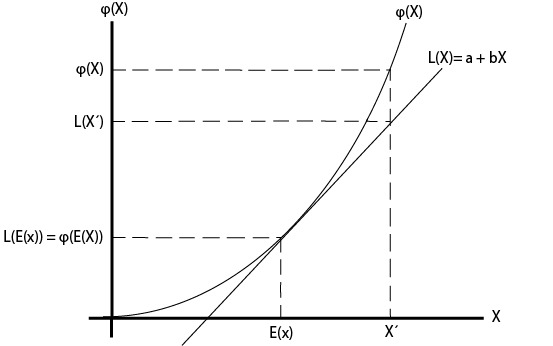
\includegraphics[scale=0.5]{img/Intuicion_Jensen.jpeg}
    \caption{Intuición geométrica de la desigualdad de Jensen }
    \label{fig:intuicion_jensen}
\end{figure}

Volviendo a lo anterior, utilizando las expresiones en \eqref{eq:total_expectation} y \eqref{eq:jensen_var}, podemos demostrar el teorema anterior.

 \begin{proof}[Demostración de Teorema \ref{teo:rao-blackwell}]
 	La varianza del estimador $\phi^\star$ está dada por 
 	\begin{alignat*}{2}
 		\Et{(\phi^\star-\theta)^2} &= \Et{(\Et{\phi|T}-\theta)^2} \quad\quad\quad &&\text{def.}\\
 								&= \Et{(\Et{\phi-\theta|T})^2}&& \text{linealidad}\\
 								&\leq \Et{\Et{(\phi-\theta)^2|T}}&& \text{Jensen}\\
 								&= \Et{(\phi-\theta)^2} &&\text{ley esperanzas totales}
 	\end{alignat*}
Donde las esperanzas exteriores son con respecto a $T$ y las interiores con respecto a $X$ (o equivalentemente a $\phi$).  Observemos además que la desigualdad anterior viene de la expresión en la ecuación \eqref{eq:jensen_var}, por lo que la igualdad es obtenida si $\V{\phi-\theta|T} = 0$, es decir, la VA $\phi-\theta$ tiene que ser constante para cada valor de $T$, es decir, $\phi$ es función de $T$. Intuitivamente podemos entender esto como que si el estadístico ya fue considerado en el estimador, entonces conocer el valor del estadístico no reporta información adicional. 
 \end{proof}

\begin{remark}
	Notemos que si el estimador $\phi$ es insesgado, su \textit{Rao-Blackwellización} $\phi^*$ también lo es, en efecto
	\begin{equation}
		\Et{\phi^*} = \Et{\Et{\phi|T}} = \Et{\phi} = \theta,
	\end{equation}
	donde la segunda igualdad está dada por la ley de esperanzas totales y la tercera por el supuesto de que $\phi$ es insesgado.
\end{remark}

\section{Varianza uniformemente mínima}

Observemos que, en base al riesgo cuadrático definido en la ecuación \eqref{eq:riesgo_cuad}, si un estimador es insesgado (Definición \ref{def:estimador_insesgado}) entonces su riesgo cuadrático es únicamente su varianza. Esto motiva la siguiente definición de optimalidad para estimadores insesgados. 

 \begin{definition}[Estimador insesgado de varianza uniformemente mínima]
  	El estimador $\phi=\phi(X)$ de $\theta$ es un estimador insesgado de varianza uniformemente mínima (EIVUM) si es insesgado y además si $\forall \phi':\cX\rightarrow \Theta$ estimador insesgado se tiene
  	\begin{equation}
  		\Vt{\phi}\leq\Vt{\phi'}, \forall \theta\in\Theta.
  	\end{equation}
  	Es decir, el EIVUM es el estimador insesgado que tiene menor varianza de todos los estimadores insesgados (y puede no ser único).
  \end{definition} 

\begin{example}
	Consideremos $X=(X_1,\ldots,X_n)\sim\ber{\theta}$ y los siguientes estimadores de $\theta$
	\begin{itemize}
		\item $\phi_1(X) = X_1$
		\item $\phi_2(X) = \frac{1}{2}(X_1+X_2)$
		\item $\phi_3(X) = \frac{1}{n}\sum_{i=1}^n X_i$
	\end{itemize}
	Observemos que todos estos estimadores son insesgados, pues como $\forall i, \Et{X_i} = \theta$, entonces 
	\begin{equation}
		\Et{\phi_1(X)} = \Et{\phi_2(X)} = \Et{\phi_3(X)} = \theta.
	\end{equation}
	Veamos ahora que la varianza de $\phi_3(X)$ está dada por
	\begin{equation}
		\Vt{\phi_3(X)} = \Vt{\frac{1}{n}\sum_{i=1}^n X_i} = \frac{1}{n^2}\sum_{i=1}^n \Vt{X_i} = \frac{\theta(1-\theta)}{n}
	\end{equation}
	pues $\Vt{X_i} = \Et{(\theta - X_i)^2} = \Et{X_i^2} - \theta^2 = (0^2 \cdot (1-\theta) + 1^2 \cdot \theta) - \theta^2 = \theta(1-\theta)$. Consecuentemente, la varianza de los estimadores considerados decae como la inversa del número de muestras $1/n$.
\end{example}

Con las definiciones anteriores, podemos mencionar el siguiente teorema, el cual conecta la noción de estadístico completo con la de EIVUM. 

\begin{theorem}[Teorema de Lehmann-Scheffé]
	Sea $X$ una VA con distribución paramétrica $\familiaparametrica$ y $T$ un estadístico suficiente y completo para $\theta$. Si el estimador $\phi = \phi(T)$ de $\theta$ es insesgado, entonces $\phi$ es el único EIVUM. 
 \end{theorem} 
 
 Es decir, el Teorema de Lehmann-Scheffé nos permite verificar que un estimador es el (único) EIVUM, si éste es insesgado y es función de un estadístico suficiente y completo. 
    

 \begin{proof}
 	Veamos en primer lugar que es posible construir un estimador en función del estadístico suficiente $\phi(T)$ que tiene menor o igual varianza que un estimador arbitrario $\phi'(X)$. En efecto, el Teorema de Rao-Blackwell establece que el estimador 
 	\begin{equation}
 		\phi(T) = \Et{\phi'(X)|T},
 	\end{equation}
 	tiene efectivamente menor (o igual) varianza que $\phi'(X)$.\\

 	Ahora veamos que solo existe un único estimador insesgado que es función del estadístico completo $T$. Asumiendo que existiesen dos estimadores insesgados de $\theta$ que son funciones de $T$, denotados $\phi_1(T),\phi_2(T)$, entonces, $\Et{\phi_1(T)-\phi_2(T)}=0$, es decir, $\phi(T) = \phi_1(T)-\phi_2(T)$ es un estimado insesgado de 0. Luego, como $T$ es completo, entonces, $\phi(T)=0$ es identicamente nulo, lo cual implica que  $\phi_1(T) = \phi_2(T)$ c.s.-$P_\theta$.\\

 	Hemos probado que (i) para un estimador arbitrario, se puede construir un estimador que es función de $T$ el cual tiene menor o igual varianza que el estimador original y, (ii) el estimador insesgado $\phi(T)$ es único. Consecuentemente, $\phi(T)$ es el único EIVUM.
 \end{proof}

El Teorema de Lehmann-Scheffé da una receta para encontrar el EIVUM: simplemente es necesario encontrar un estadístico completo y construir un estimador insesgado en base a éste, esto garantiza que el estimador construido es el \textbf{único} EIVUM.
\begin{example}[EIVUM para Bernoulli]
	Recordemos que en el Ejemplo \ref{eq:est_completo_bernoulli} vimos que el estadístico $T=\sum_{i=1}^nX_i$ es completo para $X\sim\ber{\theta}$. Como el estimador de $\theta$ dado por $\phi(T) = T/n$ es insesgado, 
\begin{equation}
	\Et{\phi(T)} = \Et{T/n} = \sum_{i=1}^n \Et{X_i} /n = \theta,
\end{equation}
entonces $\phi(T) = T/n$ es el EIVUM para $\theta$ en $\ber{\theta}$ y es único.	
\end{example}

\begin{remark}
Lectura personal: Estadístico auxiliar (ancilliary) y teoremas de Basur y de Bahadur. 
\end{remark}

\begin{definition}
Un estadístico T=T(X) se dice \textbf{ancilario} si su distribución no depende del parámetro a estimar.
\end{definition}

\begin{theorem}[Teorema de Basu]
Si T es completo y suficiente para $\theta$ y V es ancilario para $\theta$, entonces T y V son independientes
\end{theorem}


\subsection{Información de Fisher}

Para entender esta propiedad, primero definamos la función de puntaje o \textit{score function} como la {función aleatoria} definida por la derivada de la log-verosimilitud, es decir, 
\begin{equation}
	S_\theta(X) = \frac{\partial \log p_\theta(X)}{\partial\theta}.
\end{equation}

\begin{remark}
La esperanza de la función de puntaje cero. En efecto, derivando la igualdad fundamental $1 = \int_\cX p_\theta(x)\dx$ con respecto a $\theta$, obtenemos 
\begin{align}
	0 = \int_\cX \frac{\partial  p_\theta(X)}{\partial\theta} \dx = \int_\cX \frac{1}{p_\theta(X)}\frac{\partial  p_\theta(X)}{\partial\theta} p_\theta(X) \dx = \int_\cX \frac{\partial \log   p_\theta(X)}{\partial\theta} p_\theta(X) \dx = \Et{S_\theta(X)}
\end{align}
Sorprendente. 
\end{remark}

Además, veamos que al derivar por segunda vez la función de puntaje, obtenemos: 
\begin{align*}
	0 &= \int_\cX \frac{\partial}{\partial \theta }\left(\frac{\partial \log   p_\theta(X)}{\partial\theta} p_\theta(X) \right)\dx\\ 
	&= \int_\cX \left(\frac{\partial^2 \log   p_\theta(X)}{\partial\theta^2} p_\theta(X) + \frac{\partial \log   p_\theta(X)}{\partial\theta}\frac{\partial   p_\theta(X)}{\partial\theta}  \right)\dx\\
	&= \Et{\frac{\partial^2 \log   p_\theta(X)}{\partial\theta^2}} + \Et{\left(\frac{\partial \log   p_\theta(X)}{\partial\theta}\right)^2}.
\end{align*}
Cada uno de los dos términos de la ecuación anterior tiene la misma magnitud (uno es negativo y el otro es positivo), lo cual motiva la siguiente definición.

\begin{definition}[Información de Fisher]
La cantidad denotada mediante  
\begin{equation}
		I(\theta) = \Et{\left(\frac{\partial \log   p_\theta(X)}{\partial\theta}\right)^2} = 	-\Et{\frac{\partial^2 \log   p_\theta(X)}{\partial\theta^2}},
\end{equation}	
es conocida como información de Fisher. Además, como la esperanza de la función de puntaje es cero, la varianza de $I(\theta)$ puede ser expresada como 
\begin{equation}
	\Vt{S_\theta(X)} = \Et{S_\theta(X)^2} - \cancel{\Et{S_\theta(X)}^2} = \Et{\left(\frac{\partial \log   p_\theta(X)}{\partial\theta}\right)^2}.
\end{equation}
Consecuentemente, la información de Fisher también es la varianza de la función de pérdida, con lo que contamos con tres expresiones para poder calcular $I(\theta)$. 
\end{definition}

\begin{exercise}[Cálculo de la información de Fisher para Bernoulli]
	Consideremos $X\sim\ber{\theta}$, entonces, 
	\begin{align}
		I(\theta) &= -\Et{\frac{\partial^2}{\partial\theta^2}\loga{\theta^X(1-\theta)^{1-X}}}\nonumber\\
		&= -\Et{\frac{\partial^2}{\partial\theta^2} X\log\theta + \frac{\partial^2}{\partial\theta^2} 	(1-X)\loga{1-\theta}	}\nonumber\\
		&= \Et{X\theta^{-2} + (1-X)(1-\theta)^{-2}	}\nonumber\\
		&= \theta^{-1} + (1-\theta)^{-1}	\nonumber\\
		&= 	\frac{1}{\theta(1-\theta)}.
	\end{align}
\end{exercise}

\begin{exercise}[Cálculo de la información de Fisher para Poisson]
	Consideremos $X\sim\poi{\theta}$, entonces, 
	\begin{align}
		I(\theta) &= \Et{\left(\frac{\partial}{\partial\theta}\loga{\frac{\theta^Xe^{-\theta}}{X!}}\right)^2}\nonumber	\\
		&= \Et{\left( \frac{\partial}{\partial\theta}X\log\theta - \frac{\partial}{\partial\theta}\theta - \frac{\partial}{\partial\theta}\log(X!)\right)^2}\nonumber\\
		&= \Et{\left( X\theta^{-1} - 1\right)^2}\nonumber	\\
		&= \Et{ X^2\theta^{-2} -2X\theta^{-1}+ 1}\nonumber	\\
		&= (\theta+\theta^2)\theta^{-2} -2\theta\theta^{-1}+ 1\nonumber\\
		&= \theta^{-1}.\nonumber	
	\end{align}
\end{exercise}

Hasta ahora hemos calculado la función de puntaje en base a la verosimilitud de solo una una variable aleatoria. Si considerásemos la verosimilitud evaluada calculada para un conjunto de observaciones (IID), tenemos que
\begin{equation}
	S_\theta(X_1,\ldots,X_n) = \frac{\partial \log \prod_{i=1}^np_\theta(X_i)}{\partial\theta} = \sum_{i=1}^n\frac{\partial \log p_\theta(X_i)}{\partial\theta}= \sum_{i=1}^n S_\theta(X_i).
\end{equation}
De igual forma, para la información de Fisher, tenemos, 
\begin{equation}
	I_n(\theta) = \Vt{\sum_{i=1}^n S_\theta(X_i)} = n I(\theta).
\end{equation}
\begin{remark}
La expresión anterior confirma la intuición sobre la información de Fisher en cuanto a \emph{cuán informativa} es una muestra $X$ para estimar el parámetro $\theta$: Si una muestra tiene tiene una información de Fisher $I(\theta)$, entonces $n$ muestras independientes del mismo modelo tendrán  $n$ veces dicha información. 
\end{remark}

\subsection{Cota de Cramer Rao}

Veamos ahora una desigualdad interesante para la información de Fisher y su relación con estimadores. Consideremos un estimador insesgado, es decir, 
\begin{equation}
	\Et{\hat{\theta}(X)-\theta}=\int_\cX (\hat{\theta}(X)-\theta)p_\theta(X)\dx=0.
\end{equation}
Derivando esta expresión con respecto a $\theta$, obtenemos

\begin{align*}
	0 &= \frac{\partial}{\partial\theta}\int_\cX (\hat{\theta}(X)-\theta)p_\theta(X)\dx\\
	  &= -\int_\cX p_\theta(X)\dx  + \int_\cX (\hat{\theta}(X)-\theta)\frac{\partial p_\theta(X)}{\partial\theta}\dx\\
	  &= -1  + \int_\cX (\hat{\theta}(X)-\theta)\frac{\partial\log p_\theta(X) }{\partial\theta}p_\theta(X)\dx.
\end{align*}
Lo que implica que 
\begin{align*}
	1 &= \left(\int_\cX (\hat{\theta}(X)-\theta)\frac{\partial\log p_\theta(X) }{\partial\theta}p_\theta(X)\dx\right)^2\\
	&=\left(\int_\cX (\hat{\theta}(X)-\theta)\sqrt{p_\theta(X)}\sqrt{p_\theta(X)}\frac{\partial\log p_\theta(X) }{\partial\theta}\dx\right)^2\\
	&\leq\int_\cX (\hat{\theta}(X)-\theta)^2 p_\theta(X)\dx \int\left(\frac{\partial\log p_\theta(X) }{\partial\theta}\right)^2 p_\theta(X)\dx.
\end{align*}
Notemos que la primera integral es la varianza del estimador insesgado $\hat\theta$ y la segunda es la esperanza del cuadrado de la función de puntaje (o la información de Fisher). Con esto, podemos enunciar el siguiente resultado 
\begin{definition}[Cota de Cramer-Rao]
	Sea $X_1,\ldots,X_n \sim p_\theta$ y $nI(\theta)$ su información de Fisher. Entonces para todo estimador insesgado $\theta'$ tenemos 
	\begin{equation}
		\Vt{\theta'}\geq (nI(\theta))^{-1},\quad \forall \theta\in\Theta
	\end{equation}
\end{definition}
La cota de Cramer-Rao es un elemento fundamental en el estudio estadístico, pues establece que cualquier estimador insesgado tiene necesariamente una varianza que está por sobre el recíproco de la información de Fisher. Es decir, la varianza de un EIVUM se encuentra acotada inferiormente.


\section{Completitud}

Otra propiedad de los estimadores que permite estudiar su capacidad de estimar es la de \textit{completitud}. A continuación definimos esta propiedad para el caso general de un estadístico, no necesariamente un estimador.

\begin{definition}[Estadístico completo]
	Un estadístico $T(X)$ es completo si para toda función $f$, se tiene que 
	\begin{equation}
		\Et{f(T)|\theta} = 0, \forall \theta\in\Theta \Rightarrow \Probt{f(T)=0} = 1, \forall \theta\in\Theta.
	\end{equation}
	
\end{definition}



Intuitivamente entonces, podemos entender la noción de completitud como lo siguiente: un estadístico es completo si la única forma de construir un estimador insesgado de cero a partir de él es aplicándole la función idénticamente nula.  Veamos un ejemplo de la distribución Bernoulli, donde el estadístico $T(x) = \sum x_i$ es efectivamente completo. 

\begin{example}
	\label{eq:est_completo_bernoulli}
	Sea $x=(x_1,\ldots,x_n)$ observaciones de $X\sim\ber{\theta}$, recordemos que $T(x) = \sum x_i\sim\bin{n,\theta}$, por lo que la esperanza de $f(T)$ está dada por
	\begin{equation}
		\Et{f(T)} = \sum_{t=0}^n f(t)\binom{n}{t}\theta^t(1-\theta)^{n-t}= (1-\theta)^n\sum_{t=0}^n f(t)\binom{n}{t}\left(\frac{\theta}{1-\theta}\right)^t,
	\end{equation}
	es decir un polinomio de grado $n$ en $r=\theta/(1-\theta)\in\R_+$. Entonces, $\Et{f(T)} = 0,\forall\theta$, implica que necesariamente los pesos de este polinomio son todos idénticamente nulos, es decir, $f(t)=0,\forall t$, lo que a su vez implica $\Probt{f(T)=0} = 1$. Consecuentemente, $T(x) = \sum x_i\sim\bin{n,\theta}$ es un estadístico completo.
\end{example}

El concepto de completitud dice relación con la construcción de estimadores usando estadísticos, lo cual puede ser ilustrado mediante el siguiente ejemplo

\begin{example}
	Consideremos dos estimadores, $\phi_1, \phi_2$ insesgados de $\theta$ distintos, es decir, 
	\begin{equation}
	\E{\phi_1} = \E{\phi_2} = \theta, \ \Prob{\phi_1\neq \phi_2} > 0.
	\end{equation}
	Definamos ahora $\phi = \phi_1 - \phi_2$, donde verificamos que $\E{\phi} = 0, \forall \theta$, es decir, $\phi$ es un estimador insesgado de cero. Como nuestra hipótesis en la ecuación anterior dice que $\Prob{\phi_1 - \phi_2=0}>0$, de acuerdo a la definición  de estadístico completo, $\phi$ no es completo. 
\end{example}


\begin{example}[Estimador de la taza de la distribución exponencial]
	\label{ex:estimador_exponancial}
	Consideremos $X\sim Exp(\theta)$, donde $Exp(x|\theta) = \theta\exp(-\theta x),\theta>0$. Veamos en primer lugar que el estadístico trivial $T(X) = X$ es completo. En efecto, para una función cualquiera $f(\cdot)$, como $\theta>0$ tenemos
	\begin{equation}
	    \Et{f(X)} = \int_0^\infty f(x)\theta\exp(-\theta x)\d x = 0 \Rightarrow  \int_0^\infty f(x)\exp(-\theta x)\d x = 0
	\end{equation}
	con lo cual si el lado derecho de la expresión anterior se cumple  $\forall \theta$, entonces necesariamente $f(x)=0$ (¿por qué?).
	
	En segundo lugar, asumamos que existe un estimador insesgado $\ghX$ de $g(\theta) = \theta$. Es decir, 
	\begin{equation}
	\nonumber
		\Et{\ghX} = \int_0^\infty \ghx\theta\exp(-\theta x)\d x = \theta, \forall \theta,
	\end{equation}
	lo cual es equivalente a $\int_0^\infty \ghx\exp(-\theta x)\d x = 1, \forall \theta$, y también a (al derivar ambos lados de esta expresión c.r.a. $\theta$) 
	\begin{equation}
	    \int_0^\infty x\ghx\exp(-\theta x)\d x = 0, \forall \theta.
	\end{equation}

	Esta última expresión es equivalente a que $\E{X\ghX} = 0$, con lo que podemos utilizar el hecho de que $X$ es un estadístico completo para decir que la función $X\ghX=0$ c.s. $\forall \theta$, y consecuentemente $\ghX=0$ c.s. $\forall \theta$. 
	
	Hemos mostrado que el supuesto de la existencia de un estimador (denotado $\ghX$) insesgado para el parámetro del modelo exponencial $\theta>0$, resulta en la contradicción $\ghX=0$ c.s. Consecuentemente, no es posible construir estimadores insesgados para $\theta$ en la distribución exponencial.
\end{example}

\section{Ejercicios}

\begin{enumerate}

\item Considere una Muestra Aleatoria Simple (MAS) $X=(X_1,...,X_n)$ donde $X_i\sim\mathcal{N}(\mu, \sigma^2)$, $\forall i =1,...,n$ con $\mu$ y $\sigma$ son parámetros desconocidos. Se consideran al estimador de la varianza y la media como:

\[S^2 := \frac{1}{n-1}\sum\limits_{i=1}^{n}(\overline{X}_n-X_i)^2, \quad \hat{\mu} := \overline{X}_n \]
donde $\overline{X}_n$ denota al promedio de $X_1,..., X_n$, es decir  $\overline{X}_n = \frac{1}{n}\sum\limits_{i=1}^{n}X_i$. 

\begin{enumerate}
    \item Demuestre que $S^2$ y $\hat{\mu}$ son independientes.
\end{enumerate}

\item Sea $X=(X_1,...,X_n)$ una MAS de un modelo Poisson de parámetro $\lambda$. Se busca estimar insesgadamente la función generadora de momentos $M_{X}(t)=\mathbb{E}[e^{tX}]$. Para esto, siga los siguientes pasos:

\begin{enumerate}
    \item Muestre que $M_{X_i}(t)=e^{-\lambda (1-e^t)}$, con $t\in \mathbb{R}$
    \item Compruebe que $\widehat{M_{X}}(t)=e^{t X_1}$ es un estimador insesgado de $M_{X}(t)$.
    \item Muestre que el estadístico $T(X)=\sum\limits_{i=1}^{n}X_i$ tiene ley Poisson de parámetro $n \lambda$.
    \item Calcule $\mathbb{P}(X_1 =k | S=s)$. ¿Qué ley sigue?
    \item Muestre que $T(X)$ es un estadístico suficiente y completo para $\lambda$
    \item Encuentre el estimador EIVUM para $M_{X}(t)$
\end{enumerate}

\item Sea una MAS $X=(X_1,..,X_n)$ con n observaciones independientes del modelo gaussiano $\mathcal{N}(\mu,\sigma^2)$ y otra MAS $Y=(Y_1,...Y_n)$ con n observaaciones independientes del modelo gaussiano $\mathcal{N}(\nu,\sigma^2)$. Se supone que X e Y son vectores independientes y que los parámetros $\mu,$ $\nu$, $\sigma$ son desconocidos y no están sujetos a ninguna restricción.

\begin{enumerate}
    \item Plantee el modelo paramétrico relacionado a la situación planteada. Compruebe $\mathcal{P}$ pertenece a la clase exponencial y que es de rango completo en la parametrización natural.
    \item Analice los siguientes estadísticos e indique si son suficientes y/o minimales:
    \begin{itemize}
        \item $T_1=\left (\sum\limits_{i=1}^{n}X_i,\sum\limits_{i=1}^{n}Y_i,\sum\limits_{i=1}^{n}X^2_i,\sum\limits_{i=1}^{n}Y^2_i  \right )$
        \item $T_2=\left (\sum\limits_{i=1}^{n}X_i,\sum\limits_{i=1}^{n}Y_i,\sum\limits_{i,j=1}^{n}Y_iX_j  \right )$
        \item $T_3=\left (\sum\limits_{i=1}^{n}(X_i+Y_i),\sum\limits_{i=1}^{n}X_i^2,\sum\limits_{i,j=1}^{n}Y^2_i  \right )$
    \end{itemize}
    \item Muestre que $S=\left (\sum\limits_{i=1}^{n}X_i,\sum\limits_{i=1}^{n}Y_i,\sum\limits_{i,j=1}^{n}Y^2_i+X^2_i  \right )$ es un estadístico suficiente completo para $\mathcal{P}$
    \item Encuentre el EIVUM para las siguientes funciones del parámetro $\theta$:
    \begin{itemize}
        \item $g_1(\theta)=\mu +\nu$
        \item $g_2(\theta)=\mu\nu$
        \item $g_3(\theta)=\sigma^2$
    \end{itemize}
    
    
    
    
\end{enumerate}



Se suele presentar cuando un vector bidimensional (por ejemplo, el que representa la velocidad del viento) tiene sus dos componentes, ortogonales, independientes y siguen una distribución normal. Su valor absoluto seguirá entonces una distribución de Rayleigh

\item Sea $X=(X_1,...,X_n)$ una MAS de $n\in \mathbb{N}$ observaciones con $X_n\sim Unif(\theta,2\theta)$. Considere que para la MAS anterior, sus estadísticos de orden $X_{(1)},...,X_{(n)}$ poseen una densidad dada por:

\[ f_{X_{(i)}}(x)=\frac{n!}{(i-1)!(n-i)!}\frac{1}{\theta}\left (\frac{x-\theta}{\theta}  \right )^{i-1}\left (1-\left (\frac{x-\theta}{\theta}  \right )  \right )^{n-i}\quad, \quad x\in[\theta,2\theta]. \]

Se busca estimar el parámetro $\theta$. Para esto se pide lo siguiente:
\begin{enumerate}
    \item Encuentre un estadístico suficiente para $\theta$.
    \item Considere el estimador $\hat{\theta}=\frac{2}{3}X_1$. Muestre que es insesgado.
    \item Utilice el Teorema de Rao-Blackwell para encontrar un estimador $\widetilde{\theta}$ de $\theta$ con menor MSE que $\hat{\theta}$. 
    \item Demuestre que $\widetilde{\theta}$ es insesgado.
    \item Interprete $\widetilde{\theta}$
\end{enumerate}
\end{enumerate}



\chapter{Construcción de estimadores}

\section{Estimador de Máxima Verosimilitud (EMV)} % (fold)
\label{sec:estimador_de_máxima_verosimilitud}

Informalmente, el estimador de un parámetro es una función de los datos que deseamos que entregue un valor cercano al parámetro. Dada una cantidad desconocida, se hace natural la idea de buscar encontrar una \emph{buena} (y ojalá la \emph{mejor}) función de los datos que nos permita estimarla, pero ¿Qué significa que un estimador sea un buen estimador?

Dado que el parámetro $\theta$ es desconocido, calcular la distancia de un estimador $\hat\theta = \hat\theta(X)$ a este no es posible, pues de lo contrario  podríamos simplemente utilizar una función de pérdida como las definidas en el capítulo anterior.

En esta sección, veremos cómo construir estimadores usando directamente la densidad de probabilidad de la VA $X\in\cX$, donde aparece el parámetro $\theta$ y una colección de datos (o realizaciones del modelo). Para este fin la función de verosimilitud en la definición \ref{función_verosimilitud} será fundamental. Recordemos que la función de verosimilitud (del parámetro $\theta$ dados los datos $X$) es la densidad de probabilidad de los datos $X$ si el valor del parámetro fuese efactivamente $\theta$. Consecuentemente, la verosimilitud permite encontrar un estimador en base a una métrica clara: cuan probable es cada estimador de haber generado los datos. Esto da las condiciones para determinar un estimador que recibe mucha atención en la literatura estadística: 

\begin{definition}[Estimador de máxima verosimilitud (MV)]
	Sea una observación $x$ y una función de verosimilitud $L(\theta)$, el estimador de máxima verosimilitud está dado por 
	\begin{equation}
		\thetaMV = \underset{\theta}{\arg\max}\ L(\theta|x)
	\end{equation}	
\end{definition}

Claramente, el estimador de MV puede ser definido con respecto a la verosimilitud o a cualquier función no decreciente de ésta, como también pude no existir o no ser único. En particular, nos enfocaremos en encontrar $\thetaMV$ mediante la maximización de la log-verosimilitud $l(\theta) = \log L(\theta)$, la cual es usualmente más fácil de optimizar en términos computacionales o analíticos. De hecho, muchas veces incluso ignoraremos constantes de la (log) verosimilitud, pues éstas no cambian el máximo de $L(\theta)$.

\begin{example}[Máxima verosimilitud: Bernoulli]
	\label{ex:bernoulli_MV}
	Sea $X_1,\ldots X_n\sim\ber{\theta}$, la verosimilitud de $\theta$ está dada por 
	\begin{equation}
		L(\theta) = \prod_{i=1}^n\theta^x_i(1-\theta)^{1-x_i},
	\end{equation}
	y su log-verosimilitud por $l(\theta) = (\sum_{i=1}^nx_i)\log \theta + (n-\sum_{i=1}^nx_i)\log(1-\theta)$. El estimador de  MV puede ser encontrado resolviendo $\frac{\partial l(\theta)}{\partial \theta} = 0$:
	\begin{align*}
	\frac{\partial l(\theta)}{\partial \theta} =0 
	&\Rightarrow  (\sum_{i=1}^nx_i) \theta^{-1} = (n-\sum_{i=1}^nx_i)(1-\theta)^{-1}\\
	&\Rightarrow  \sum_{i=1}^nx_i (1-\theta) = (n-\sum_{i=1}^nx_i) \theta\\
	&\Rightarrow  \theta = \sum_{i=1}^nx_i/n.
	\end{align*}
Notemos que este estimador de MV ¡es a su vez el EIVUM!	
\end{example}


\begin{exercise}
	Graficar $l(\theta)$ en el Ejemplo \ref{ex:bernoulli_MV}.
\end{exercise}

\begin{exercise}
	Encuentre el estimador de MV de $\theta = (\mu,\Sigma)$ para la VA $X\sim\cN(\mu,\Sigma)$.
\end{exercise}

\begin{example}
	Sea la VA $X\sim\uni{\theta}$, es decir, $p(x) = \theta^{-1} \ind_{0\leq x \leq \theta}$. Para calcular la verosimilitud, recordemos en primer lugar que la verosimilitud factoriza de acuerdo a  
	\begin{equation}
		L(\theta) = \prod_{i=1}^n p_\theta(x_i)
	\end{equation}
	y observemos que necesariamente $p_\theta(x_i) = 0$ si $x_i>\theta$. Consecuentemente, $L(\theta)>0$ solo si $\theta$ es mayor que toda las observaciones, en particular, si $\theta\geq\max\{x_i\}_1^n$.

	Además, si efectivamente tenemos $\theta\geq\max\{x_i\}_1^n$, entonces notemos que $p_\theta(x_i) = 1/\theta$, por lo que la verosimilitud está dada por
		\begin{equation}
		L(\theta) = \theta^{-n}, \quad \theta\geq\max\{x_i\}_1^n
	\end{equation}
	y consecuentemente, el estimador de máxima verosimilitud es $\thetaMV = \max\{x_i\}_1^n$.
\end{example}

\section{Propiedades del EMV} 
\label{sec:propiedades_EMV}

\subsection{Consistencia} 

La primera propiedad que veremos del EMV es su consistencia. Que un estimador $\hat\theta$ sea \textit{consistente} quiere decir que éste tiende (de alguna forma) al parámetro real $\theta$ a medida vamos considerando más datos. Recordar en lo siguiente que la KL hace referencia a la divergencia de Kullback-Leibler.


 Con la KL, definiremos que un modelo/parámetro es \textbf{identificable} si los valores para los parámetros $\theta\neq\theta'$ implican $\KL{p_\theta}{p_\theta'}>0$, lo que significa que distintos valores del parámetro dan origen a distintos modelos, intuitivamente, esto significa que la \emph{parametrización} del modelo estadístico no es redundante. Asumiremos desde ahora que los modelos considerados son identificables.

El estimador de MV puede ser obtenido de la maximización de
\begin{equation}
\label{eq:Mn}
 	M_n (\theta') = n^{-1} (l_n(\theta') - l_n(\theta))  = \frac{1}{n} \sum_{i=1}^n \loga{\frac{p_{\theta'}(x_i)}{p_{\theta}(x_i)}},
 \end{equation} 
 donde $n$ es la cantidad de observaciones $\{x_1,\ldots,x_n\}$, $\theta$ es el parámetro real y $l_n(\cdot)$ es la log-verosimilitud en base a dichas observaciones. La obtención del EMV desde la maximización de $M_n (\theta')$ en la ecuación \eqref{eq:Mn} es posible porque $l_n(\theta)$ es constante para $\theta'$, con lo que $l_n(\theta')\propto_{\theta}M_n (\theta')$. 
 
 Entonces, gracias a la ley de los grandes números, tenemos que 
 \begin{equation}
 	M_n(\theta') \rightarrow \Et{\loga{\frac{p_{\theta'}(x)}{p_{\theta}(x)}}} = -\Et{\loga{\frac{p_{\theta}(x)}{p_{\theta'}(x)}}} = -\KL{p_\theta}{p_{\theta'}}.
 \end{equation}

 Consecuentemente, como el objetivo del estimador de MV tiende a la KL negativa, entonces maximizar la verosimilitud es equivalente a minimizar la KL-divergencia entre el modelo real y el modelo generado por el parámetro. 
\begin{remark}
 Máxima verosimilitud es (asintóticamente) efectivavamente equivalente a minimizar discrepancias en el espacio de modelos.
\end{remark}
 
\begin{remark}
 Si el modelo obtenido mediante MV tiende efectivamente al modelo real (no tenemos garantías de esto todavía) nuestro supuesto de \textit{identificabilidad} implica que el estimador de MV tiende al parámetro real también. Sin embargo, si el modelo está parametrizado de tal forma que no es identificable, convergencia en el espacio de modelos no implica necesariamente convergencia en los parámetros.   
\end{remark}
 
 


 Otra propiedad muy utilizada en la práctica es el \textbf{Principio de equivarianza}, el cual establece que si $\thetaMV$ es el estimador de MV de $\theta$, entonces, $g(\thetaMV)$ es el estimador de MV del parámetro transformado $g(\theta)$.

\begin{example}(Cálculo del EMV en Gaussiana: varianza versus precisión versus log-precisión versus cholesky - reparametrisation trick)
	
\end{example}

\subsection{Normalidad asintótica}

Otra propiedad es la \textbf{normalidad asintótica del EMV}, esto significa que el estimador ML (como cantidad aleatoria) es normal en el límite que la cantidad de  observaciones tiende a infinito. 

Formalmente, si tenemos una colección de VA $X_1,\ldots,X_n\sim p_\theta$ con $\theta$ el parámetro real, entonces, la secuencia de estimadores de MV, $\thetaMV^{(n)}$ cumple con 
\begin{equation}
	\sqrt{n}(\thetaMV^{(n)}-\theta)\rightarrow \cN(0,(I(\theta))^{-1}),
\end{equation}
lo cual intuitivamente corresponde a que, para $n$ suficientemente grande, el estimador de MV está distribuido de forma normal en torno al parámetro real con varianza $(nI(\theta))^{-1}$. Lo que implica también \textit{eficiencia asintótica}: si $n$ es suficientemente grande, entonces la distribución del estimador es normal y su varianza tiende a cero. Es decir, asintóticamente, el EMV alcanza la Cota de Cramer Rao para la varianza. 


\section{Estimador de Mínimo Cuadrático Ordinario (MCO)}

El Estimador de Mínimo Cuadrático Ordinario (MCO) es un tipo de aproximación de mínimos cuadrados mediante una función lineal de los datos. Formalmente, supongamos que se busca predecir $Y_i\in\mathbb{R}$ con $i=1,...,n$ donde $n$ representa la cantidad de datos mediante una función lineal de los datos $(X_i) \in R^{k}$, es decir, mediante una ponderación y suma de $k$ variables. Se asume que $X_{i1}=1,\forall i$ para considerar un intercepto y que existe un error $\epsilon_i$ de estimación para cada dato. Con esto, el modelo lineal viene dado por:

$$
Y_i= \sum_{j=1}^{k}\beta_j X_{ij} + \varepsilon_i
$$
con $\mathbb{E}(\varepsilon_i)=0$. En forma matricial, se considera que:
$$
Y=\begin{pmatrix}
Y_1 \\
Y_2\\
\vdots\\
Y_n\\
\end{pmatrix} ; 
X= \begin{pmatrix}
X_1 \\
X_2\\
\vdots\\
X_n\\
\end{pmatrix}
\quad
\beta= \begin{pmatrix}
\beta_1 \\
\beta_2\\
\vdots\\
\beta_k\\
\end{pmatrix} \text{ y }
\varepsilon= \begin{pmatrix}
\varepsilon_1 \\
\varepsilon_2\\
\vdots\\
\varepsilon_n\\
\end{pmatrix}
$$

Recordar que para fila de $X\in \R^{n \times k }$ es una observación. Con esto, el modelo lineal en su forma matricial viene dado por: 
$$
Y=X\beta + \varepsilon
$$

\begin{definition}[Estimador de Mínimo Cuadrático Ordinario (MCO)]

La idea es buscar una solución del sistema $X\beta=Y$, el cual generalmente no tiene solución, por lo cual se busca una aproximación para $\beta$. Bajo la siguiente función de costo:

\[S(\beta)=\sum\limits_{i=1}^{n}|y_i-\sum\limits\limits_{i=1}^{n}X_{ij}\beta_{j}|^2=||Y-X\beta||^2\]

el estimador $\hat{\beta}$ viene dado por:

\[\hat{\beta}=\argmin_\beta S(\beta)\]

el cual tiene como solución, si es que $X^{T}X$ es invertible, dada por:

$$
\hat{\beta}= (X^{T}X)^{-1}X^{T}Y
$$

Cuando se cumplen las siguientes condiciones:
\begin{itemize}
    \item Exogenedidad: $\mathbb{E}[\varepsilon|X]=0$, 
    \item Homocedasticidad: $\mathbb{E}[\varepsilon^2_i|X]=\sigma^2 $
    \item No autocorrelación: $\mathbb{E}[\varepsilon_i\varepsilon_j|X]=0,\forall i\neq j$.
\end{itemize}

se entiende a $\hat{\beta}$ como el estimador de mínimos cuadrados ordinarios (MCO, o OLS por su nombre en ingles), en donde además:
$$
\mathbb{V}(\hat{\beta})= \sigma^{2}(X^{T}X)^{-1}
$$
\end{definition}

\subsection{Teorema de Gauss-Markov}

\begin{prop}
El estimador $\hat{\beta}$ es insesgado, es decir, $\mathbb{E}[\hat{\beta}|X]=\beta$
\end{prop}

\begin{theorem}][Teorema de Gauss-Markov]
Si es que se cumple homocedasticidad y no autocorrelación de los errores para el estimador MCO, se tiene que el estimador $\hat{\beta}$ es eficiente en la clase de estimadores lineales insesgados. Lo anterior se denomina un estimador lineal insesgado óptimo (ELIO), o en su nombre en ingles, best linear unbiased estimator (BLUE). Esta eficiencia es en el sentido de que, sea $\bar{\beta}$ otro estimador lineal e insesgado de $\beta$, entonces se tiene que:

\[\mathbb{V}[\hat{\beta}|X]-\mathbb{V}[\bar{\beta}]\leq 0\]
\end{theorem}
es decir, el estimador MCO $\hat{\beta}$ es el estimador linear insesgado con menor varianza. 




\section{Regresión}

La palabra \emph{regresión} fue introducida por Francis Galton (1822-1911), haciendo referencia a que los hijos de personas altas, tendían a ser más bajos que sus padres,  fenómeno que denominó \textbf{Regresión a la media}. Este mismo fenómeno se puede observar cuando la segunda película de una saga no es tan buena como la primera parte. \\
La regresión es un método para estudiar la relación entre una variable $Y$, y otra variable independiente $X$, denominada característica. 
\begin{definition}[Función de Regresión] Se define la función de regresión $r(x)$ como:
$$
r(x)=\mathbb{E}(Y|X=x)=\int yf(y|x)dx
$$

\end{definition}
La idea de este método consiste en, dados datos $\mathcal{D}=\left \{ x_i,y_i \right \}_{i=1}^{n}$, encontrar una distribución $F_{X,Y}$. 


\subsection{Regresión Lineal Simple}

Comencemos viendo el caso unidimensional, es decir $X_i \in \R$. Buscamos ajustar $r(x)$ de forma tal que: 
$$
r(x)=\beta_0 + \beta_1 x,
$$

 es decir, de forma que y sea una función lineal (o lineal a fin ) de x. 
Supondremos que hay un ruido $\varepsilon_i$ tal que $\mathbb{V}(\varepsilon_i)=\sigma^2$, y es independiente de $x$. \\
\begin{definition}
Se define el modelo de regresión lineal simple como: 
$$
Y_i=\beta_0+\beta_1 X_i+ \varepsilon_i,
$$
con $\mathbb{E}(\varepsilon_i)=0$, y $\mathbb{V}(\varepsilon_i)=\sigma^2$.
\end{definition}
Buscamos estimar $\beta_0$ y $\beta_1$ de forma que tengamos una aproximación lineal que sea lo mejor posible. Estas últimas palabras nos hacen preguntarnos ¿Los mejores estimadores con respecto a qué? La respuesta es, con respecto a la métrica de mínimo cuadrados: 
$$
J(\hat{\beta_0},\hat{\beta_1})=\dfrac{1}{2} \sum_{i=1}^{n}(Y_i-\hat{Y_i})^{2},
$$
donde $\hat{Y_i}=\hat{\beta_0}+\hat{\beta_1}X_i$. 
\begin{theorem}
Los estimadores de mínimos cuadrados son: 
$$
\hat{\beta_1}=\dfrac{\sum_{i=1}^{n}(X_i-\bar{X})(Y_i-\bar{Y_i})}{\sum_{i=1}^{n}(X_i-\bar{X})^{2}}
$$
$$
\hat{\beta_0}=\bar{Y}-\hat{\beta_1}\bar{X}
$$
Un estimador insesgado de $\sigma^2$ es:
$$
\hat{\sigma^2}=\dfrac{1}{n-2} J(\hat{\beta_0},\hat{\beta_1})
$$
\end{theorem}

\subsection{Mínimos Cuadrados y Máxima Verosimilitud}
Supongamos ahora que $\varepsilon \sim \mathcal{N}(0,\sigma^2$, es decir, 
$Y_i|X_i \sim \mathcal{N}(\mu_i,\sigma^2)$, con $\mu_i=\beta_0 + \beta_1 X_i$.
Calculemos la verosimilitud: 
$$
\mathcal{L}=\prod_{i=1}^{n}f_{X}(X_i) f_{Y|X}(Y_i|X_i)= \prod_{i=1}^{n}f_{X}(X_i) \prod_{i=1}^{n}f_{Y|X}(Y_i|X_i)
$$
Llamemos $\mathcal{L}_1$ a la primera parte de este producto, y $\mathcal{L}_2$ a la segunda parte. Como $\mathcal{L}_1$ no depende de $\beta_0 $ y $\beta_1$, tenemos que para calcular los estimadores de máxima verosimilitud de estos parámetros, nos importa el segundo parámetro. Entonces, considerando la log-verosimilitud de $\mathcal{L}_2$:

$$ \mathcal{L}_2 = \prod_{i=1}^{n} f_{Y|X}(Y_i|X_i) \propto \sigma^{-n} exp(\dfrac{-1}{2\sigma^2}\sum_{i} (Y_i-\mu_i)^2) 
$$ 
$$
\implies l=-nlog(\sigma)-\dfrac{-1}{2\sigma^2}\sum_{i=1}^{n}(Y_i-(\beta_0 + \beta_1 X_i)^2
$$
Notemos que al minimizar esto, como el primer término es constante con respecto a $\beta_0 $ y $\beta_1$, tenemos: 
\begin{theorem}
Bajo la hipótesis de normalidad, el estimador de mínimos cuadrados coincide con el estimador de máxima verosimilitud. También se tiene: 
$$
\hat{\sigma}^2=\dfrac{1}{n} \sum_{i=1}^{n}(Y_i-\hat{Y_i})
$$
\end{theorem}
\begin{remark}
El estimador anterior de $\hat{\sigma}^2$ normalmente se reemplaza por el estimador insesgado de la parte anterior. 
\end{remark}



\begin{remark} Podemos tener observaciones de muchos $X_i$, pero no incluirlos todos al modelo. Un modelo más reducido tiene dos ventajas: La primera es que puede entregar mejores predicciones que un modelo más grande, y la segunda es que es más simple.\\  
Generalmente, mientras más variables se añaden a la regresión, el sesgo de la predicción disminuye pero aumenta la varianza. Una muestra pequeña genera mucho sesgo; esto se llama \emph{underfitting}. Una muestra muy grande lleva a una alta varianza; esto se llama \emph{overfitting}. Las buenas predicciones vienen de balancear sesgo y varianza. 
\end{remark}

\subsection{Regresión Logística}

\begin{definition}
Se llama función logística a la función: 
$$
f(x)=\dfrac{e^x}{1+e^x}
$$
\end{definition}
\begin{figure}[h]
    \centering
    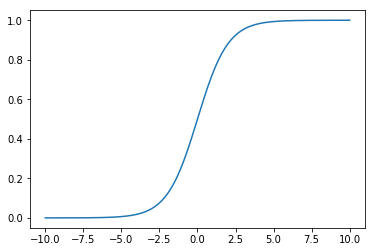
\includegraphics[scale=0.65]{img/funcion_logistica.png}
    \label{fig:logistica}
    \caption{Función Logística}
\end{figure}
La regresión logística es un método de regresión para el caso en que $Y_i \in \left \{0,1 \right \}$. El modelo considera: 

$$
p_i \equiv p_i(\beta) \equiv \mathbb{P}(Y_i=1 | X=x)= f(\beta_0+\sum_{j=1}^{k}\beta_{j} x_{ij}),
$$ 

con $f$ la función logística. De forma equivalente, si definimos $logit(p)=log(\dfrac{p}{1-p})$: 

$$
p_i=logit(p_i)= \beta_0+\sum_{j=1}^{k}\beta_j x_{ij}
$$

Como $Y_i$ son variables binarias, se tiene que   $Y_i|X_i=x_i \sim Ber(p_i)$. Así, la función de verosimilitud será:
$$
\mathcal{L}=\prod_{i=1}^{n} p_i(\beta)^{Y_i}(1-p_i(\beta))^{1-Y_i}
$$
Obtenemos el estimador de $\beta$, $\hat{\beta}$ usando método numéricos de optimización. 

\subsection{Sobre Regresión LinealEMV en práctica: tres ejemplos}
\label{sub:MV_tres_ejemplos}

\subsubsection{Regresión lineal y gaussiana} 
\label{sub:reg_lin}


Una aplicación muy popular del estimador de MV es en los modelos de regresión lineal y gaussianos. Consideremos el caso donde se desea modelar la cantidad de pasajeros que mensualmente viajan en una aerolínea, para esto, sabemos de nuestros colaboradores en la división de análisis de datos de la aerolínea que ésta cantidad tiene una tendencia de crecimiento cuadrática en el tiempo y además una componente oscilatoria de frecuencia anual. Estos fenómenos pueden ser explicados por el aumento de la población, los costos decrecientes de la aerolínea y la estacionalidad anual de las actividades económicas. 

Asumiendo que la naturaleza de la cantidad de pasajeros es estocástica, podemos usar los supuestos anteriores para modelar la densidad condicional  de dicha cantidad (con respecto al tiempo $t$) mediante una densidad normal parametrizada de acuerdo a 
\begin{equation}
	X \sim \cN\left(\theta_0 + \theta_1 t^2 + \theta_2\cos(2\pi t/12), \theta_3^2\right),
\end{equation}
donde $\theta_0,\theta_1,\theta_2$ parametrizan la media y $\theta_3$ la varianza. 

Consecuentemente, si nuestras observaciones están dadas por $\{(t_i,x_i)\}_{i=1}^n$ podemos escribir la log-verosimilitud de $\theta$ como 
\begin{align}
	\label{eq:logV_ejemplo_reg}
	l(\theta) 	&=\loga{\prod_{i=1}^n \frac{1}{\sqrt{2\pi\theta_3^2}}\expo{-\frac{(x_i-\theta_0 - \theta_1 t^2 - \theta_2\cos(2\pi t/12))^2}{2\theta_3^2}}}\nonumber \\
	&=\frac{n}{2}\loga{2\pi\theta_3^2}  - \frac{1}{2\theta_3^2}\sum_{i=1}^n (x_i - \theta_0 - \theta_1 t_i^2 - \theta_2\cos(2\pi t_i/12))^2
\end{align}
con lo que vemos que $\thetaMV$ puede ser calculado explícitamente y es función de $\{(t_i,x_i)\}_{i=1}^n$ debido a que la ecuación \eqref{eq:logV_ejemplo_reg} es cuadrática en $[\theta_0,\theta_1,	\theta_2]$.


% subsection estimador_de_mv_en_la_práctica_tres_ejemplos (end)

\subsubsection{Regresión no lineal: clasificación} 
\label{sub:clasif}

La razón por la cual $\thetaMV$ pudo ser calculado de forma explícita es porque el modelo Gaussiano con media parametrizada de forma lineal resulta en una log-verosimilitud cuadrática, donde el mínimo es único y explícito. Sin embargo, en muchas situaciones el modelo lineal y gaussiano no es el apropiado. 

Un ejemplo es esto es problema de evaluación crediticia (\textit{credit scoring}) donde en base a un conjunto de \textit{características} que definen a un cliente, un ejecutivo bancario debe evaluar si otorgarle o no el crédito que el cliente solicita. Para tomar esta decisión, el ejecutivo puede revisar la base de datos del banco e identificar los clientes que en el pasado pagaron o no pagaron sus créditos para determinar el perfil del \textit{pagador} y el del \textit{no-pagador}. Finalmente, un nuevo cliente puede ser \textit{clasificado} como pagador/no-pagador en base su similaridad con cada uno de estos grupos. 

Formalmente, denotemos las características del cliente como $t\in\R^N$ y asumamos que el cliente paga su crédito con probabilidad $\sigma(t)$ y no lo paga con probabilidad $1- \sigma(t)$, la función $\sigma(t)$ a definir. Esto es equivalente a construir la VA $X$
\begin{equation}
 	X|t \sim \ber{\sigma(t)}
 \end{equation} 
 donde $X=1$ quiere decir que el cliente paga su crédito y $X=0$ que no. Una elección usual para la función $\sigma(\cdot)$ es la función logística aplicada a una transformación lineal de $t$, es decir, 
 \begin{equation}
 	\Pr{(X=1|t)} = \frac{1}{1+e^{-(\theta_0 + \theta_1 t)	}}.
 \end{equation}
Notemos que este es un clasificador lineal, donde $\theta = [\theta_0, \theta_1]$ define un hiperplano en $\R^N$ en donde los clientes $t\in\{t | 0\leq \theta_0 + \theta_1 t\}$ pagan con probabilidad mayor o igual a 1/2 y el resto con probabilidad menor o igual a 1/2. Esto es conocido como \textbf{regresión logística}. 

Entonces, usando los registros bancarios $\{(x_i,t_i)\}_{i=1}^n$ ¿cuál es el $\theta = [\theta_0, \theta_1]$ de máxima verosimilitud? Para esto notemos que la log-verosimilitud puede ser escrita como 
\begin{align*}
	l(\theta) &= \log \prod_{i=1}^n p(x_i|t) \\
			  &= \sum_{i=1}^n x_i \log \sigma(t) + \left(n-\sum_{i=1}^n x_i\right)\log(1-\sigma(t))\\
			  &= \sum_{i=1}^n x_i \log \frac{1}{1+e^{-(\theta_0 + \theta_1 t)	}} + \left(n-\sum_{i=1}^n x_i\right)\log(1-\frac{1}{1+e^{-(\theta_0 + \theta_1 t)	}})
\end{align*}
Esta expresión no tiene mínimo global y a pesar que podemos calcular su gradiente, no podemos resolver $\partial l(\theta)/\partial \theta =0$ de forma analítica, por lo que debemos usar métodos de descenso de gradiente.  

\subsubsection{Variables latentes: \textit{Expectation-Maximisation}} 
\label{sub:EM}

En ciertos escenarios es natural asumir que nuestros datos provienen de una mezcla de modelos, por ejemplo, consideremos la distribución de estaturas en una población, podemos naturalmente modelar esto como una mezcla de distribuciones marginales para las estaturas de hombres y mujeres por separado, es decir, 
\begin{equation}
	X\sim p\cN(X|\mu_H,\Sigma_H) + (1-p)\cN(X|\mu_M,\Sigma_M)
\end{equation}
donde la verosimilitud de los parámetros $\theta = [p, \mu_H, \sigma_H,, \mu_M, \sigma_M]$ dado un conjunto de observaciones $\{x_i\}_{i=1}^n$ es
\begin{align*}
	L(\theta) 	&= \prod_{i=1}^n \left( p\cN(X|\mu_H,\Sigma_H) + (1-p)\cN(X|\mu_M,\Sigma_M) \right)\\
				&= \prod_{i=1}^n \left( p\frac{1}{\sqrt{2\pi\Sigma_H^{-1}}}\expo{\frac{-(x_i-\mu_H)^2}{2\Sigma^2_H}} + (1-p)\frac{1}{\sqrt{2\pi\Sigma_M^{-1}}}\expo{\frac{-(x_i-\mu_M)^2}{2\Sigma^2_M}}\right).
\end{align*}
Optimizar esta expresión con respecto a las 5 componentes de $\theta$ es difícil, en particular por la suma en la expresión, lo cual no permite simplificar la expresión mediante la aplicación de $\log(\cdot)$. 

Una interpretación de la diferencia de este modelo con respecto a los anteriores es la introducción implícita de una  \textit{variable latente} que describe de qué gaussiana fue generada cada observación. Si conociésemos esta variable latente, el problema sería dramáticamente más sencillo. En efecto, asumamos que tenemos a nuestra disposición las observaciones $\{z_i\}_{i=1}^n$ de la VA $\{Z_i\}_{i=1}^n$ las cuales denota de qué modelo es generada cada observación, por ejemplo, $Z_i=0$ (cf. $Z_i=1$) denota que el individuo con estatura $X_i$ es hombre (cf.~mujer).
 
En este caso, asumamos por un segundo que estas variables latentes están disponibles y consideremos los \textbf{datos completos} $\{(x_i,z_i)\}_{i=1}^n$ para escribir la función de verosimilitud completa mediante
\begin{align*}
	l(\theta|z_i,x_i) &= \prod_{i=1}^n \cN(X|\mu_H,\Sigma_H)^{z_i} \cN(X|\mu_M,\Sigma_M)^{(1-z_i)}\\
	&\hspace{-3em}= \sum_{i=1}^n \left( z_i\log\frac{1}{\sqrt{2\pi\Sigma_H^{-1}}}\expo{\frac{-(x_i-\mu_H)^2}{2\Sigma^2_H}} + (1-z_i)\log\frac{1}{\sqrt{2\pi\Sigma_M^{-1}}}\expo{\frac{-(x_i-\mu_M)^2}{2\Sigma^2_M}}\right).
\end{align*}
Esta función objetivo es mucho más fácil de optimizar, pero no es observable pues la VA $Z$ es desconocida. Una forma de resolver esto es tomando la esperanza condicional de la expresión anterior (con respecto a $Z$) condicional a los datos y los parámetros \textit{actuales}, para luego maximizar esta expresión c.r.a. $\theta$ y comenzar nuevamente. Específicamente, como la expresión anterior es lineal en $z_i$ basta con tomar su esperanza: 
\begin{align*}
	\Et{Z_i|\theta_t,x_i} &= 1\cdot\Prob{Z_i=1|\theta_t,x_i} + 0\cdot\Prob{Z_i=0|\theta_t,x_i}\\
	&= 	\frac{\Prob{x_i|\theta_t,z_i=1} p(z_i=1)}{p(x_i|\theta)}\\
	&= 	\frac{\Prob{x_i|\theta_t,z_i=1} p(z_i=1)}{p(x_i|z=1,\theta)p(z=1)+p(x_i|z=0	,\theta)p(z=0)}
\end{align*}

\section{Método de los Momentos}

Sean $X_1,...,X_n$ $n$ muestras i.i.d. de una variable aleatoria $X$ con función de densidad $p_X(x;\theta)$ o $f_X(x;\theta)$ en el caso de ser discreta o continua respectivamente, dependientes de un parámetro $\theta\in\mathbb{R}^k$ a estimar.

Recordar que los momentos de una variable aleatoria viene dado por $\mu_k=\mathbb{E}[X^k]$ donde $k$ representa el $k$-momento.

El estimador del método de los momentos es un estimador $\hat{\theta}\in\mathbb{R}^k$ de $\theta$ como la solución (si es que existe) de las $k$ ecuaciones simultaneas de los primeros $k$ momentos, esto es:

\begin{align*}
    \mathbb{E}[X^1]&=\dfrac{1}{n}\sum\limits_{i=1}^{n}x_i\\
    \mathbb{E}[X^2]&=\dfrac{1}{n}\sum\limits_{i=1}^{n}x_i^2\\
    \vdots\\
    \mathbb{E}[X^k]&=\dfrac{1}{n}\sum\limits_{i=1}^{n}x_i^k\\
\end{align*}

\begin{example}][Caso Exponencial]
Consideremos $X_1,...,X_n$ $n$ muestras i.i.d. de una variable aleatoria $X\sim exp(\theta)$ donde claramente $k=1$. Aplicando el método de los momentos, debemos resolver que:
\[\mathbb{E}[X]=\dfrac{1}{n}\sum\limits_{i=1}^{n}x_i\]

Por lo que 
\[\mathbb{E}[X]=\dfrac{1}{\theta}=\dfrac{1}{n}\sum\limits_{i=1}^{n}x_i\]

y entonces:

\[\hat{\theta}=\dfrac{1}{\dfrac{1}{n}\sum\limits_{i=1}^{n}x_i}\]

el cual calza justamente con el estimador EMV de $\theta$. 
\end{example}


\section{Intervalos de Confianza} 

En distintas situaciones, la estimación puntual de un parámetro puede no ser apropiada e incluso inverosímil, mientras que la distribución posterior puede ser poco interpretable por el público general. En dichos casos, es recomendable identificar un rango donde, con cierta probabilidad, el parámetro real está contenido. Esto motiva la siguiente definición: 

\begin{definition}[Intervalo de confianza]
\label{def:conf_inter} Un $(1-\alpha)$-intervalo de confianza para el parámetro $\theta$ fijo y desconocido, $\alpha\in[0,1]$, es el intervalo aleatorio $(A(X),B(X))$ tal que 
\begin{equation}
	\label{eq:conf_inter}
	\Probt{A(X)\leq\theta\leq B(X)} = 1-\alpha, \forall \theta\in\Theta.
\end{equation}
\end{definition}

\begin{remark}
	La definición del intervalo de confianza no describe una probabilidad sobre el parámetro $\theta$, pues estamos tomando un enfoque frecuentista (no bayesiano) donde éste es fijo. Por el contrario, lo que es aleatorio en la ecuación \eqref{eq:conf_inter} es el intervalo, no el parámetro. Entonces, si bien es una sutileza, la definición anterior se debe entender como la probabilidad de que ``el intervalo (aleatorio) contenga al parámetro (fijo)'', y no como la probabilidad de que ``el parámetro esté en el intervalo''. 
\end{remark}
Una consecuencia clave de este concepto es que si $I_{1-\alpha}$ es un $(1-\alpha)$-intervalo de confianza, entonces si fuese posible repetir una gran cantidad de veces el ejercicio de recolectar datos $X$ y calcular este intervalo para cada una de estas observaciones, entonces el parámetro $\theta$ estaría contenido en el intervalo un $100(1-\alpha)\%$ de las veces. Esto es muy diferente de asegurar que para un solo experimento, la probabilidad de que el parámetro $\theta$ esté contenido en $I_{1-\alpha}$ es $1-\alpha$, lo cual no es cierto. Los siguientes ejemplos tienen por objetivo ayudar a aclarar este concepto.

Para la construcción de intervalos de confianza es crucial la siguiente definición:

\begin{definition}[Pivote]

Sea $X=(X_1,...,X_n)$ una muestra aleatoria simple de una variable aleatoria cualquiera de depende de un parámetro $\theta$, el cual puede ser escalar o un vector. Sea $g(X,\theta)$ una variable aleatoria cuya distribución sea la misma para cualquier valor de $\theta$. A la función $g$ se de llama pivote.

\end{definition}

Veamos un ejemplo de la construcción de un pivote para el caso de la variable aleatoria normal.

\begin{example}[Intervalo de confianza para la media de la distribución normal]
	Consideremos la muestra $X_1,\ldots,X_n\sim\cN(\theta,1)$. Como $\bar{X}=\frac{1}{n}\sum_{i=1}^nX_i\sim\cN(\theta,1/n)$ tenemos que  
	\begin{equation}
			\sqrt{n}(\bar{X}-\theta)\sim\cN(0,1).
		\end{equation}	
	Esta cantidad es un \emph{pivote}. Consecuentemente, podemos identificar directamente un intervalo de confianza para el pivote desde una tabla de valores para la distribución normal de media cero y varianza unitaria. Si $\phi(x)$ denota la distribución Normal, entonces podemos elegir  $x_1$ y $x_2$ tal que $\phi(x_2)-\phi(x_1) = 1-\alpha$ con lo que tenemos
	\begin{equation}
	 	\Probt{x_1 \leq \sqrt{n}(\theta-\bar{X}) \leq x_2} = 1-\alpha \Leftrightarrow \Probt{\bar{X} + x_1/\sqrt{n} \leq \theta \leq \bar{X} + x_2/\sqrt{n}} = 1-\alpha,
	 \end{equation} 
	 es decir, $(\bar{X} + x_1/\sqrt{n},\bar{X} + x_2/\sqrt{n})$ es el $(1-\alpha)$-intervalo de confianza para $\theta$. 
	 
	 Eligiendo $\alpha=0.05$ una alternativa es tenemos $x_2 = -x_1 =1.96$, con lo que el intervalo de confianza del 95\% para $\theta$ está dado por 
	 \begin{equation}
	 	(\bar{X} -1.96/\sqrt{n},\bar{X} + 1.96/\sqrt{n}).
	 \end{equation}

	 El procedimiento estándar para encontrar intervalos de confianza es como el ilustrado en el ejemplo anterior, en donde construimos una cantidad que tiene una distribución que no depende del parámetro desconocido (llamada pivote). Construir un intervalo de confianza para esta cantidad es directo desde las tablas de distribuciones, luego, podemos encontrar el intervalo de confianza para la cantidad deseada, e.g., el parámetro desconocido, mediante transformaciones de la expresión del pivote. 

	 \begin{remark}
	 	El intervalo de confianza no es único. Por ejemplo, en el caso gaussiano podemos elegir en intervalo centrado en cero o desde $-\infty$. Esta elección dependerá de las aplicación en cuestión: una regla general es elegirlo de forma centrada para densidades que son simétricas, centrado en la moda para distribuciones unimodales, mientas que para densidades con soporte positivo podemos elegirlo desde cero. 
	 \end{remark}

	 Hasta ahora hemos solo definido intervalos de confianza para cantidades escalares, en donde el concepto de intervalo tiene sentido. Para parámetros vectoriales, nos referiremos a  \textit{conjuntos de confianza}. Siguiendo la Definición \ref{def:conf_inter}, un $(1-\alpha)$-conjunto de confianza $S(X)$ es tal que 
	 \begin{equation}
	\label{eq:conf_set}
	\Probt{\theta\in S(X)} = 1-\alpha, \forall \theta\in\Theta.
\end{equation}
\end{example}


\begin{exercise}
Considere $X_1,\ldots,X_{50}\sim\cN(0,\sigma^2)$, calcule el intervalo de confianza del 99\% para $\sigma$.
\end{exercise}

\begin{example}[Intervalo de confianza ---aproximado--- para Bernoulli] Consideremos $X_1,\ldots,X_{n}\sim\ber{\theta}$ y calculemos un intervalo de confianza para $\theta$. Recordemos que el EMV es $\thetahat = \frac{1}{n}\sum_{i=1}^nX_i$ y debido a la normalidad asintótica del EMV, tenemos que para $n$ grande, podemos asumir 
\begin{equation}
	\thetahat\sim\cN\left(\theta,\frac{\theta(1-\theta)}{n}\right),
\end{equation}
donde la varianza $\frac{\theta(1-\theta)}{n}=I_n(\theta)^{-1}$ es la inversa de la información de Fisher. 

Podemos entonces considerar el pivote
\begin{equation}
	\frac{\sqrt{n}(\thetahat-\theta)}{\sqrt{\theta(1-\theta)}}\sim\cN(0,1),
\end{equation}
y calcular el $(1-\alpha)$-intervalo de confianza asumiendo los valores $x_1$ y $x_2$ mediante 
\begin{align*}
	\Probt{x_1 \leq \tfrac{\sqrt{n}(\theta-\thetahat)}{\sqrt{\theta(1-\theta)}} \leq x_2} = 1-\alpha \Leftrightarrow \Probt{\thetahat + \tfrac{x_1\sqrt{\theta(1-\theta)}}{\sqrt{n}} \leq \theta \leq \thetahat + \tfrac{x_2\sqrt{\theta(1-\theta)}}{\sqrt{n}}} = 1-\alpha.
\end{align*}
Sin embargo, los bordes de este intervalo no son conocidos, pues dependen de $\theta$. Una forma de aproximar el intervalo es reemplazar el parámetro por su EMV. 
\end{example}


\begin{exercise}[Encuesta de elecciones presidenciales] Considere una encuesta que ha consultado a 1000 votantes y su candidato ha recibido 200 votos. Use el resultado del ejemplo anterior para determinar el intervalo de confianza del 95\% de la cantidad de votos que su candidato obtendría en la elección presidencial. 
\end{exercise}

Finalmente, revisaremos el siguiente ejemplo, el cual pretende ejemplificar el concepto de que en solo un experimento, la determinación del $(1-\alpha)$-intervalo de confianza no quiere decir que la probabilidad de que el parámetro esté contenido en él es $(1-\alpha)$\%. 

\begin{example}[Intervalo de confianza para una distribución uniforme]
\label{eq:unif_int_conf}Considere $X_1,X_2\sim\uni{\theta-\tfrac{1}{2},\theta+\tfrac{1}{2}}$ y observe que 
\begin{align*}
	\Probt{\min(X_1,X_2) \leq \theta \leq \max(X_1,X_2)} 
		&= \Probt{ X_1 \leq \theta \leq X_2}  + \Probt{ X_2 \leq \theta \leq X_1} \\
		&= \frac{1}{2}\times \frac{1}{2} + \frac{1}{2}\times\frac{1}{2}\\
		&= \frac{1}{2}
\end{align*}
corresponde al intervalo del 50\%. 

Sin embargo, si observáramos $X_1 = x_1$ y $X_2 = x_2$ tal que $|x_1-x_2|\geq\tfrac{1}{2}$ entonces necesariamente está contenido en el intervalo $(\min(X_1,X_2) , \max(X_1,X_2))$ con probabilidad 1. Esto ilustra la idea de que, en un experimento dado, la probabilidad de que $\theta$ esté en intervalo de confianza del $(1-\alpha)$\% no es necesariamente $(1-\alpha)$\%.
\end{example}


\section{Ejercicios}

\begin{enumerate}
    \item Se quiere estudiar el comportamiento de un vector bidimensional que tiene sus dos componentes ortogonales, independientes y que siguen una distribución normal. Al realizar las mediciones respectivas de cada componente, se obtiene una Muestra Aleatoria Simple (MAS, cada dato es generado desde una misma distribución y son independientes entre sí (iid)) $U=(U_1,...,U_n)$ de $n$ observaciones con $U_n\sim\mathcal{N}(0,\sigma^2)$  y una MAS $W=(W_1,...,W_n)$  de $n$ observaciones con $W_n\sim\mathcal{N}(0,\sigma^2)$. En específico, se busca estudiar el comportamiento de los módulos de los vectores obtenidos. Se obtiene una nueva MAS $X=(X_1,...,X_n)$ dada por:

\[X_i = \sqrt{U_i^2 - W_i^2}\]

\begin{enumerate}
    \item [i.] Encuentre la función de densidad de $X_1$\\
    \item Encuentre un estadístico suficiente para $\sigma^2$.
    \item Encuentre un estadístico suficiente minimal para $\sigma^2$.
    \item Encuentre el Estimador de Máxima Verosimilitud de $\sigma^2$.
    \item ¿Es el estimador $\widehat{\sigma^2}_{EMV}$ insesgado? Si no lo es, modifíquelo para que así sea.
    \item Encuentre un EIVUM de $\sigma^2$.
    \item Encuentre la distribución de  $\sqrt{n}(\widehat{\sigma^2}_{MLE}-\sigma^2)$
\end{enumerate}

\item Estudiaremos la varianza $\sigma^2$ de una Muestra Aleatoria Simple (MAS) $X=(X_1,...,X_n)$ donde $X_i\sim\mathcal{N}(\mu, \sigma^2)$, $\forall i =1,...,n$. Se considera que $\mu$ y $\sigma$ son parámetros desconocidos. 

Considere el siguiente estimador de la varianza dado por:

\[S^2 := \frac{1}{n-1}\sum\limits_{i=1}^{n}(\overline{X}_n-X_i)^2\]
donde $\overline{X}_n$ denota al promedio de $X_1,..., X_n$, es decir  $\overline{X}_n = \sum\limits_{i=1}^{n}X_i$. 
\begin{enumerate}
    \item [i.] Demuestre que $\mathbb{E}(S^2) = \sigma^2$ 
    \item [ii.] Calcule la varianza de $S^2$, para esto encontraremos primero la distribución de $\frac{n-1}{\sigma^2}S^2$, siga los siguientes pasos:
    \begin{enumerate}
        \item [ii.a.] Desarrolle la expresión $W=\sum\limits_{i=1}^{n}\frac{(X_i-\mu)^2}{\sigma^2}$ para llegar a:
        \[W = \frac{(n-1)}{\sigma^2}S^2  + \frac{n(\overline{X}_n-\mu)^2}{\sigma^2} \]
        \item [ii.b.] Encuentre las distribuciones asociadas a W y a $\frac{n(\overline{X}_n-\mu)^2}{\sigma^2} $
        \item [ii.c.] Aplique la función generadora de momentos en ambos lados de la ecuación. Para esto, asuma que $S^2$ es independiente de $\overline{X}_n$.
        \item [ii.d.] Encuentre la distribución de $\frac{n-1}{\sigma^2}S^2$
        \item [ii.e.] Calcule $\mathbb{V}(S^2)$
    \end{enumerate}
    \item [iii.] (Ejercicio) Calcule la varianza de $S^2$ desarrollando \textit{a mano} (Muy largo). 
\end{enumerate}


Ahora se considera otro estimador de la varianza dado por:

\[\hat{\sigma}^2 := \frac{1}{n}\sum\limits_{i=1}^{n}(\overline{X}_n - X_i)^2    \]

\begin{enumerate}
    \item [iv.] Muestre que $\hat{\sigma}^2$ cumple que $\mathbb{E}(\hat{\sigma}^2) \neq \sigma^2$ 
    \item [v.] Muestre que $\hat{\sigma}^2$ cumple que $\lim\limits_{n\rightarrow \infty} \mathbb{E}(\hat{\sigma}^2) = \sigma^2$
\end{enumerate}

\begin{enumerate}
    \item [vi.] Calcule $ECM_{\sigma^2}(S^2)$
    \item [vii.] Calcule $ECM_{\sigma^2}(\hat{\sigma}^2) $
    \item [viii.] Verifique que $ECM_{\sigma^2}(\hat{\sigma}^2) < ECM_{\sigma^2}(S^2)$
\end{enumerate}

\item \item Sea $X=(X_1,...,X_n)$ una MAS con una función de densidad dada por:
    \begin{equation}
        \nonumber 
        f(x|\theta)=\theta x^{\theta -1},\theta>0,x\in (0,1)
    \end{equation}
    \begin{itemize}
        \item Encuentre el estimador MLE para $\theta$. Calcule su esperanza y su varianza. ¿Cómo se comporta la varianza asintoticamente?
    
    \item[(vii)] ¿Es $\hat{\theta}_{MLE}$ insesgado para $\theta$? Si no lo es, modifíquelo con tal de que sea insesgado.
    
    \item[(viii)] Calcule el ECM de $\hat{\theta}_{MLE}$ y del estimador encontrado en la parte anterior. Basado en el criterio ECM, ¿Cúal de los dos estimadores es preferible?
    
    \item[(iX)] Denotemos como $\theta^{\star}$ al estimador encontrado en la parte (vii). ¿$\theta^{\star}$ alcanza la Cota de Cramer-Rao?
    
    \item[(X)] Si el estimador $\theta^{\star}$ no alcanza la Cota de Cramer Rao, ¿Tenemos que buscar un mejor estimador insesgado para $\theta$?
    \end{itemize}
    
    \item Sea $X=(X_1,...,X_n)$ una MAS con una función de densidad dada por:
\begin{equation}
    \nonumber 
    f(x|\theta)=\frac{2x}{\theta^2},\theta>0,0<x\leq \theta
\end{equation}

\begin{itemize}
    \item[(i)] Encuentre un estadístico suficiente para $\theta$.
    
    \item[(ii)] Encuentre un estadístico minimal suficiente para $\theta$.
    
    \item[(iii)] Encuentre el estimador MLE para $\theta$
    
    \item[(iv)] Calcule el ECM de $\hat{\theta}_{MLE}$
    
    \item[(v)] Si $\hat{\theta}_{MLE}$ es sesgado, modifíquelo para que sea insesgado. Denotémoslo como $\theta^{\star}$
    
    \item[(vi)] ¿Es $\theta^{\star}$ el mejor estimador insesgado de $\theta$?
\end{itemize}

\item Estudios relacionados con el comportamiento de ciertos bichos indican que estos tienden a organizarse al azar, linealmente, en un intervalo de longitud $\theta > 0$, a la derecha de un punto donde se ubica una feromona. Nos gustaría estimar el valor del parámetro $\theta$. Sea $X=(X_1,...,X_n)$ una muestra aleatoria simple (MAS) de la distancia de n bichos con respecto a la feromona.

\begin{enumerate}
    \item Defina el modelo paramétrico correspondiente.
    \item Considere el estimador $\hat{\theta}=2\Bar{X_n}$. ¿Será insesgado? Si no lo es, modifíquelo para que lo sea.
    \item Ahora, considere el estimador $\hat{\theta}=\max\{ X_1,...,X_n\}$. ¿Será insesgado? Si no lo es, modifíquelo para que lo sea.
    \item Calcule el ECM para cada uno de los estimadores y compárelos.
\end{enumerate}

\item
Considere un modelo lineal dado por $y_i=\beta x_i +\epsilon_i$ con $i=1,...,n$. Se tiene que $\epsilon_i$ son i.i.d. con $\mathbb{V}(\epsilon_i))=\sigma^2$, $\mathbb{E}(\epsilon_i)=0$ y que $X_i\perp \epsilon_i$, $\forall i$. Para estimar $\beta$ se han sugerido los siguientes estimadores:

\[\hat{\beta_1}=\frac{\sum\limits_{i=1}^{n}y_i}{\sum\limits_{i=1}^{n}x_i} \qquad\hat{\beta_2}=\frac{\sum\limits_{i=1}^{n}x_i y_i}{\sum\limits_{i=1}^{n}x_i} \]
Estudie el sesgo de cada estimador. Calcule la varianza de cada uno de los estimadores y compárelos con la varianza del estimador de MCO.

\item Considere el modelo lineal en forma matricial dado por:
\[Y=X\beta +\epsilon\]
Con $\beta\in\mathbb{R}^k$, $\mathbb{E}(\epsilon)=0_{nx1}$ y $\mathbb{V}(\epsilon)=\sigma^2Id_{n}$, con $\sigma$ un parámetro desconocido. Pruebe las siguientes propiedades del modelo:

\begin{itemize}
    \item $X^t\epsilon=0$
    \item $Y^tY=\hat{Y}^t\hat{Y}+\hat{\epsilon}^t\hat{\epsilon}$
    \item $\hat{\epsilon}^t\hat{\epsilon}=Y^tY-\hat{\beta}X^tY$
\end{itemize}

\item \textbf{Un poco de Geometría}
Llamemos $E_X$ al espacio generado por las columnas de X. Llamemos $P_X$ a la matriz que proyecta a un vector de $\mathbb{R}^n$ en el espacio generado por las columnas de X. Llamemos $E_{X^{\perp}}$ al espacio ortogonal a $E_X$. Se puede demostrar que la matriz que proyecta en el espacio generado por las columnas de X y la proyección en el ortogonal vienen dadas por:

\[P_X=X(X^tX)^{-1}X^t  \qquad P_{X^{\perp}}=Id- X(X^tX)^{-1}X^t  \]
Escriba los siguientes en términos de $P_X$ y $P_{X^{\perp}}$
\begin{itemize}
    \item $\hat{\epsilon}=Y-X\hat{\beta}$
    \item $\hat{Y}=P_X Y$
\end{itemize}
Se postula el siguiente estimador para la varianza de los errores $\sigma^2_\epsilon$:
\[\hat{\sigma_\epsilon^2}=\hat{\epsilon}^t\hat{\epsilon}\]
Escriba el estimador en términos de $P_X$ y $P_{X^{\perp}}$ y estudie su sesgo.
\end{enumerate}


